\documentclass[letterpaper,11pt]{article}
\usepackage[american]{babel}

\usepackage[hidelinks]{hyperref}

% I like international letters
\usepackage[utf8]{inputenc}

\usepackage[authordate,strict,sorting=nyt,babel=other,cmsdate=both]{biblatex-chicago}
\usepackage{mathtools}
\bibliography{UCSB-GEOG172}

\usepackage{fancyhdr}
\pagestyle{fancy}
\lhead{\emph{Matthew Wigginton Conway}}
\rhead{\emph{\today}}

\usepackage{graphicx}

\usepackage{geometry}

\usepackage{listings}
\lstset{language=R,breaklines=true}

\newcommand{\reflst}[1]{#1 (page \pageref{#1})}

\title{Analyzing the Effects of Space and Time on Bikeshare Use: A Case Study in Washington, DC}
\author{Matthew Wigginton Conway}
\date{\today}

\begin{document}
\fancyhfoffset[E,O]{0pt}
\maketitle

Bikesharing is a relatively new form of shared transportation wherein
bikes are deposited at stations throughout a city. Users pay an annual
fee and they can then take bikes from any station and return them to
any station. These systems generate a wealth of data. The stations are
electronic, so each time a trip is taken, a record is stored in a
database with the origin, destination, start and end times of that
trip. For some systems, this data is freely available online. This
project aims to use data on the approximately 4.5 million trips taken
on Washington, DC's Capital Bikeshare (CaBi) system from 2010 through the
present to examine how time of day and station location affect the
usage of the bikeshare system.

\section{Data Processing}

Before analysis could be undertaken, the data needed to be obtained
and cleaned.  The data are available from the CaBi
website\footnote{\url{http://capitalbikeshare.com/system-data}} as a
series of quarterly CSV files. Data from the fourth quarter of 2010
through the 2nd quarter of 2013 were used. Each record contains the
origin and destination of the trip, the start and end times, and
ancillary information.  The script \reflst{fetchData.sh} was used to
download the CSV files. The files were then merged using
\reflst{csvMerge.py}. This script also cleaned the data; the column
names in the CSV files from different quarter differ slightly, so the script
contains code to normalize them.  It also renames the columns to
remove whitespace, making it simpler to use the data in R.

There are no spatial data present in the trip history files. To remedy
this, station locations were retrieved from the CaBi real-time
API\footnote{\url{http://capitalbikeshare.com/data/stations/bikeStations.xml}}
and merged with the trip history data using
\reflst{expandFileWithXY.py}.\marginpar{discuss stations with no geo
  coordinates}

Finally, \reflst{load\string_data.R} was used to load the data into R,
removing trips longer than 20km or 2 hours, assuming these trips to
be errors.

\section{Time of Day Effects}

One of the chief difficulties of any bikeshare system is keeping
bicycles balanced across the system. The problem is doubly
constrained, because the system operator not only needs to keep enough
bikes available at all stations, but also needs to prevent stations
from becoming completely full and thus preventing people from parking
the bikes. This is usually accomplished via a fleet of trucks which
pick up bikes from overfull stations and rebalance them to empty or
nearly empty stations.

For the time of day portion of this project, the data on bike share
trips was used to determine whether the distribution of start and end
stations differs significantly between time periods. Eight time
periods were defined: morning (6a--9a), midday (9a--3p), afternoon
(3p--7p) and overnight (7p--9p) for both weekdays and weekends. The
boundaries of the time periods are the same as those used in the
Metropolitan Washington Council of Governments travel model, although
MWCOG does not further divide the time periods into weekday and
weekend patterns \autocite[14]{MWCOG2013}.

\subsection{Methodology}

Each trip in the data was first assigned a time period based on its
start time using \reflst{labeling.R}. For each time period, an
origin-destination matrix was created, showing the number of trips
between each station pair using \reflst{relabel.R}. The matrices were
then compared pairwise, comparing each time period to every other time
period. The following test statistic was computed for each pairwise
comparison.

\begin{equation}\label{eq:timets}
 \displaystyle\sum_i \sum_j (t_{ij,1} - t_{ij,2})^2 \over
 (\displaystyle \sum_i \sum_j t_{ij,2})^2
\end{equation}

Where $i$ and $j$ represent origin and destination stations,
respectively, $t_{ij,1}$ is trips from origin $i$ to destination $j$
in time period 1, and $t_{ij,2}$ is trips from origin $i$ to
destination $j$ in time period 2. The denominator of the equation is
to scale the test statistic based on the total number of trips taken
in the time period, so that the magnitude of the test statistic is not
affected by the absolute number of trips taken in the time
period. Additionally, matrix 2 is scaled before calculation such
that the total number of trips in each matrix are the same. That is,

\begin{equation}\label{eq:timeconstraint}
  \displaystyle \sum_i \sum_j t_{ij,1} = \sum_i \sum_j t_{ij,2}
\end{equation}

Once test statistics were computed for each pair of time periods, a
Monte Carlo simulation was undertaken to determine whether the time
periods differ significantly. The trips that were originally used to
generate the origin-destination were randomly reassigned to different
time periods. The number of trips in each time period was held
constant. Since this worked by relabeling the existing trips, the
distribution of trips to origins and destinations was constant over
all time periods though it varied within time
periods. Origin-destination matrices were then calculated using the
relabeled trips, and the same pairwise comparison was done and test
statistics computed. This process was repeated 999 times. This
simulation was performed by \reflst{relabel.R}.

\subsection{Results}

It was found that there is an effect of time of day on the
origin-destination matrices. For every pair, there was no test
statistic from the Monte Carlo simulation higher than the test statistic
from the observed pair. The p-values between time periods are show below.

\noindent \begin{footnotesize}
\begin{tabular}{p{3cm} | l l l l l l l l}
& WkMr & WkMd & WkAf & WkNt & WeMr & WeMd & WeAf & WeNt \\
\hline
Weekday Morning (6a--9a)   & 0.999 & 0.000* & 0.000* & 0.000* & 0.000* & 0.000* & 0.000* & 0.000* \\
Weekday Midday (9a--3p)    & 0.000* & 0.999 & 0.000* & 0.000* & 0.000* & 0.000* & 0.000* & 0.000* \\
Weekday Afternoon (3p--7p) & 0.000* & 0.000* & 0.999 & 0.000* & 0.000* & 0.000* & 0.000* & 0.000* \\
Weekday Overnight (7p--6a) $\dagger$ & 0.000* & 0.000* & 0.000* & 0.999 & 0.000* & 0.000* & 0.000* & 0.000* \\
Weekend Morning (6a--9a)   & 0.000* & 0.000* & 0.000* & 0.000* & 0.999 & 0.000* & 0.000* & 0.000* \\
Weekend Midday (9a--3p)    & 0.000* & 0.000* & 0.000* & 0.000* & 0.000* & 0.999 & 0.000* & 0.000* \\
Weekend Afternoon (3p--7p) & 0.000* & 0.000* & 0.000* & 0.000* & 0.000* & 0.000* & 0.999 & 0.000* \\
Weekend Overnight (7p--6a) $\dagger$ & 0.000* & 0.000* & 0.000* & 0.000* & 0.000* & 0.000* & 0.000* & 0.999 \\
\hline
\multicolumn{9}{l}{* Statistically significant at $\alpha = 0.05$ level} \\
\multicolumn{9}{l}{$\dagger$ Friday night is a weekend night, Sunday night is a weekday night.} \\
\end{tabular}
\end{footnotesize}


The p-value represents the probability that the observed differences
between two time periods could have occurred by chance. As we can see,
there is a statistically significant difference between every time
period and every other time period ($p < 0.05$).

\subsection{Discussion}

Such a result should not be surprising. To take a trivial example,
commuters may ride from a residential area to a Metro stop each
morning, and the reverse each evening. Weekend trips may represent
people using the system for pleasure or entertainment rather than
commuting. The data confirm that usage patterns (measured by station
origin-destination matrices) differ for each time period.

This intensifies the need for rebalancing. Bikeshare demand is often
not in equilibrium, so bikes must be moved from station to station by
the system operator in order to ensure that there are available bikes
and available docks at all stations \autocite[108]{IDAE2007}. That is,
if most people ride bikes from residential areas to commercial areas
in the morning, there will not be enough bikes available in
residential areas, and there will not be enough docks available in
commercial areas. The problem is doubly-constrained, because there
need to both be bikes available at each station in order for users to
take a bike, and empty docks in order to return bikes. An interesting
project would be to determine to what extent demand is cyclical. If
the demand is cyclical, with people biking to commercial areas in the
morning and back to residential areas in the afternoon, providing a
sufficient number of bikes would ameliorate the need for rebalancing.
There may, however, be a general trend as well. For instance, people
may prefer to bikeshare to work if they are in a hurry and bikeshare
is faster than transit\footnote{Using this same trip history data, it
  was found that many trips in the data are faster than comparable
  bikeshare trips; people tend to use bikeshare for trips where it is
  faster than transit \autocite{Wong2012}.}, and take transit
home if they are tired. In this case, there could be a general trend
of bikes moving towards commercial areas. This could be tested using
the trip history data, but is beyond the scope of this project.

\section{Effects of Space on Bikeshare Use}

Some bike share stations are, of course, more popular than others. It
was hypothesized that station popularities (defined here as the
average number of bike movements---both pickups and dropoffs---per
day) are spatially autocorrelated. That is, stations near each other
would tend to have similar popularities. To test this, a Moran's $I$
statistic was computed to evaluate whether there is significant
autocorrelation between station popularities.

\subsection{Methodology}

Data were loaded into R, and were then summarized to get a count of
bike movements for each station. This process was repeated twice to
get counts for both the number of trips originating and the number of
trips terminating at each station; the results were then summed by
station. This number of bike movements was then normalized by dividing
by the number of days each station had been open. The count of bike
movements is skewed right, with many stations having relatively few
bike movements per day, and a few stations having a large number of
bike movements per day. In order to better analyze the data, a Box-Cox
transformation was undertaken to normalize the distribution. Using the
Shapiro-Wilks estimator, the Box-Cox parameter was estimated as
$\lambda = 0.33$. This did serve to make the distribution more
symmetric (see fig. \ref{fig:boxcox} for a comparison between the
untransformed and transformed distribution). The transformed
distribution, however, is bimodal. This should not affect the Moran's
$I$ calculation, however, but explanation of this would be a
worthwhile direction for future research.

\begin{figure}[t]
  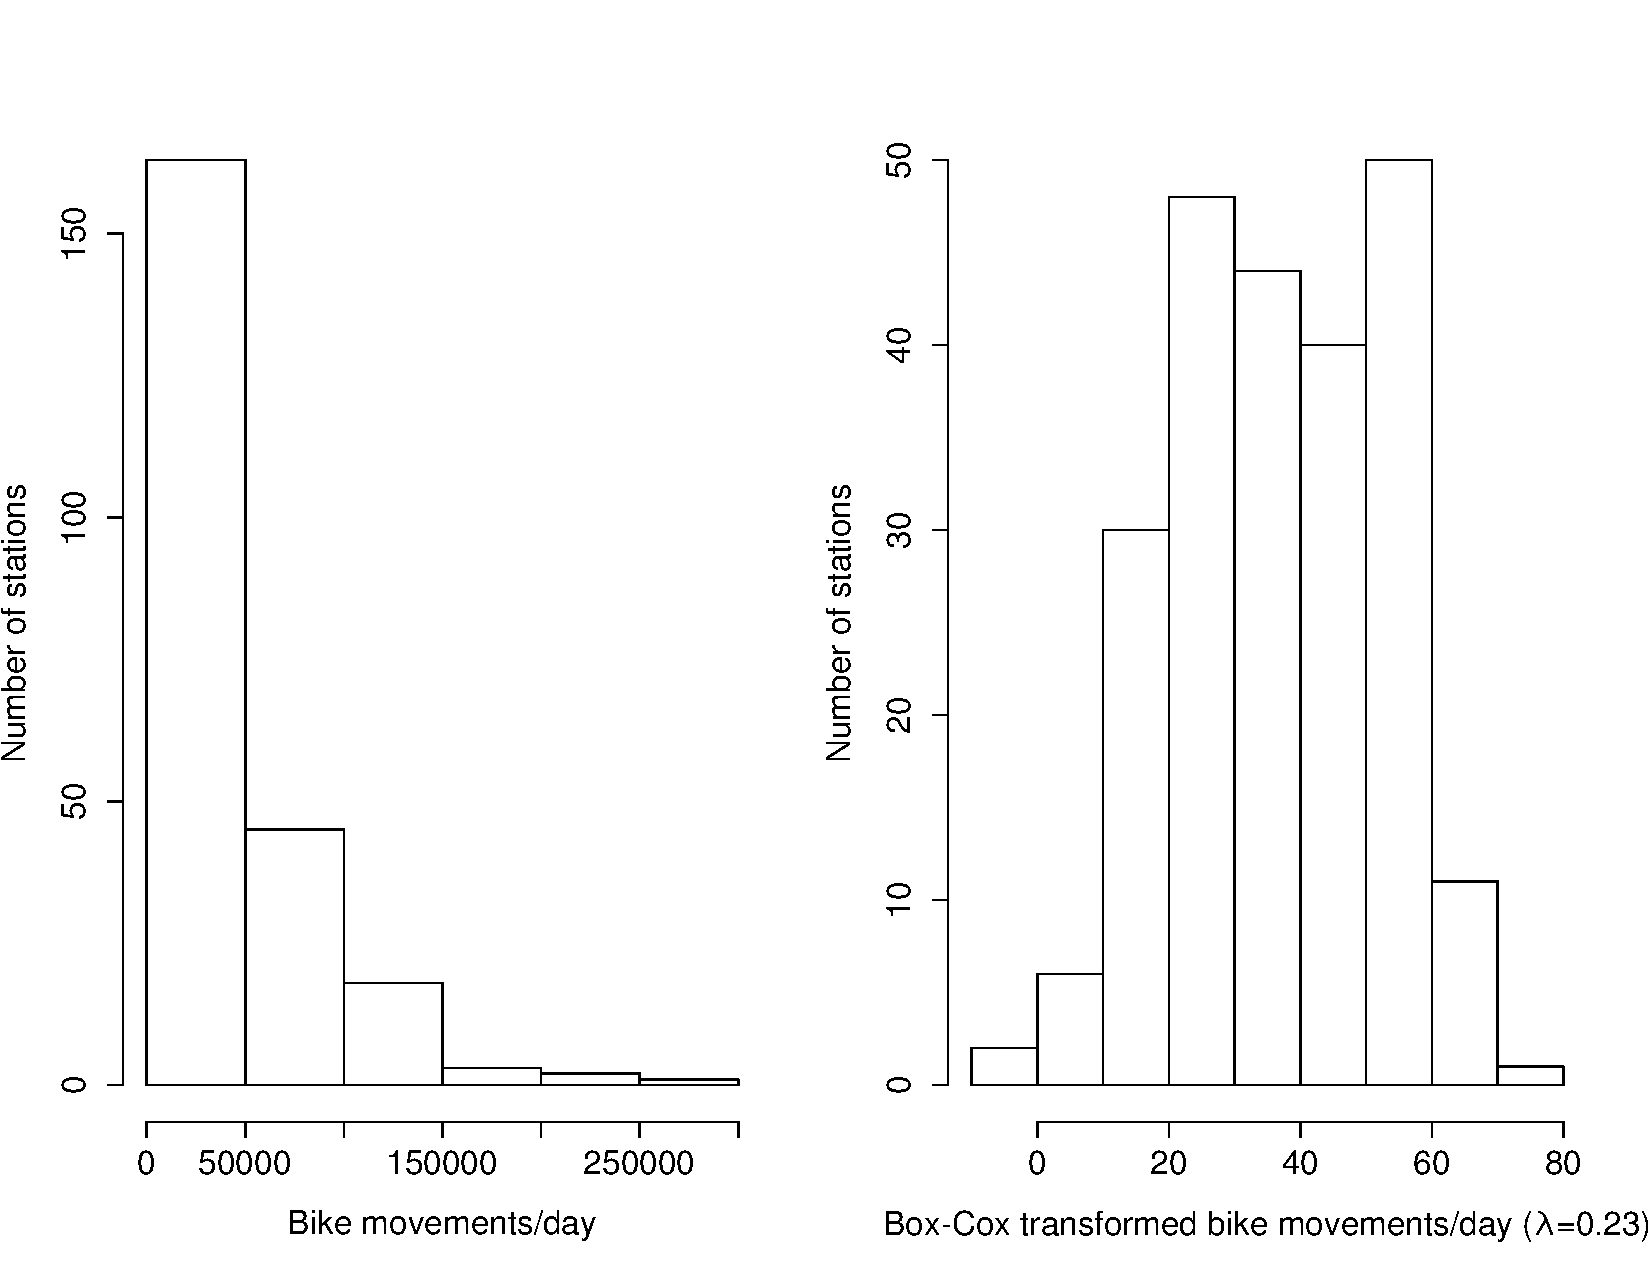
\includegraphics[width=\textwidth]{boxcox.pdf}
  \caption{\label{fig:boxcox}Station popularity, before and after Box-Cox transformation.}
\end{figure}

\begin{figure}[t]
  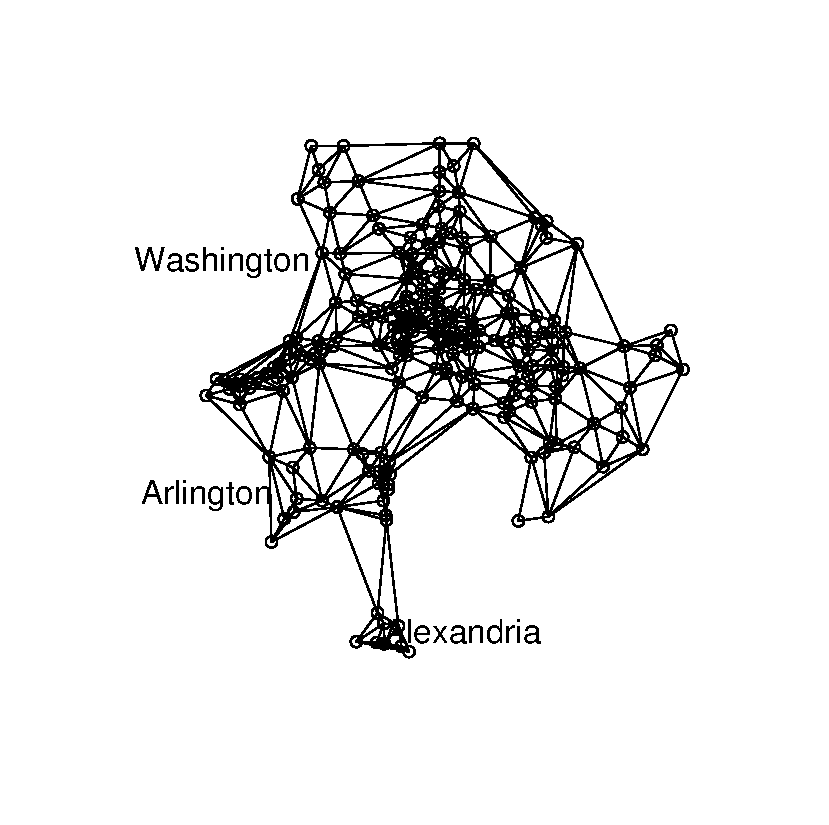
\includegraphics[width=\textwidth]{connectivity_labels.pdf}
  \caption{\label{fig:nbmat} Station adjacency graph: Delaunay triangulation with links
    longer than 4km removed.}
\end{figure}

\begin{figure}[t]
  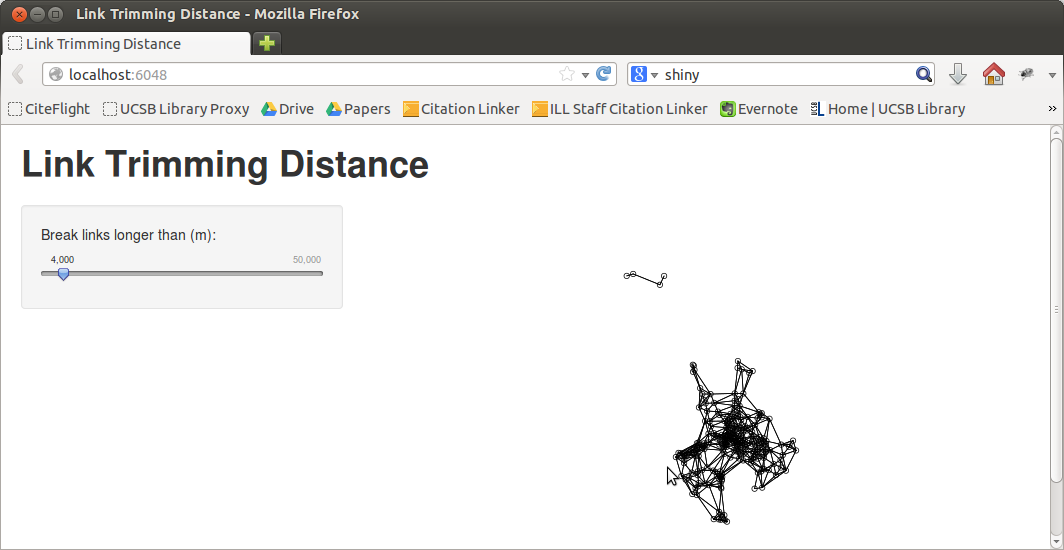
\includegraphics[width=\textwidth]{shiny.png}
  \caption{\label{fig:shiny} A Shiny application for interactively
    visualizing networks with different link lengths; adjusting the
    slider changes the maximum link length in the network, breaking
    more or fewer links in the original triangulation.}
\end{figure}


To calculate $I$, a weight matrix was first calculated. This was done
by creating a Delaunay triangulation of the stations using the
\texttt{tri2nb} function from the \texttt{spdep} package. Links longer
than 4km were removed, which left two graph components, one in
Washington, Arlington and Alexandria, and one in Montgomery County,
Maryland. The component in Montgomery County was removed for the
purposes of this analysis. 4km was chosen as a the maximum link length
visually, removing the most outrageous links while still keeping some
degree of connectivity. A Shiny application was created to visualize the
network with different thresholds for breaking links; a slider can be
used to adjust the threshold while seeing results in real time (see
Figure \ref{fig:shiny}, \reflst{server.R} and \reflst{ui.R}). The
adjacency graph defined is shown in figure \ref{fig:nbmat}.

The adjacency graph was then converted to a weight matrix in
row-standardized form (that is, all rows sum to 1). Thus the
neighborhood value of a point can be interpreted as a local
mean. Moran's $I$ was calculated, and a Moran plot was generated for
further interpretation.

\subsection{Results}

A Moran's $I$ value of 0.78 was found ($p < 0.05$), indicating strong
positive spatial autocorrelation between stations. That is, stations
near each other tend to have similar popularities. Upon examining the
Moran plot (fig. \ref{fig:moran}), we see clearly the positive
trend. We also see that the influential points (marked
\rlap{\tiny{+}}{$\diamond$}) are fairly evenly distributed about the
scatter. These influential points are somewhat spatially dispersed as
well (see fig. \ref{fig:map}).

\begin{figure}[t]
  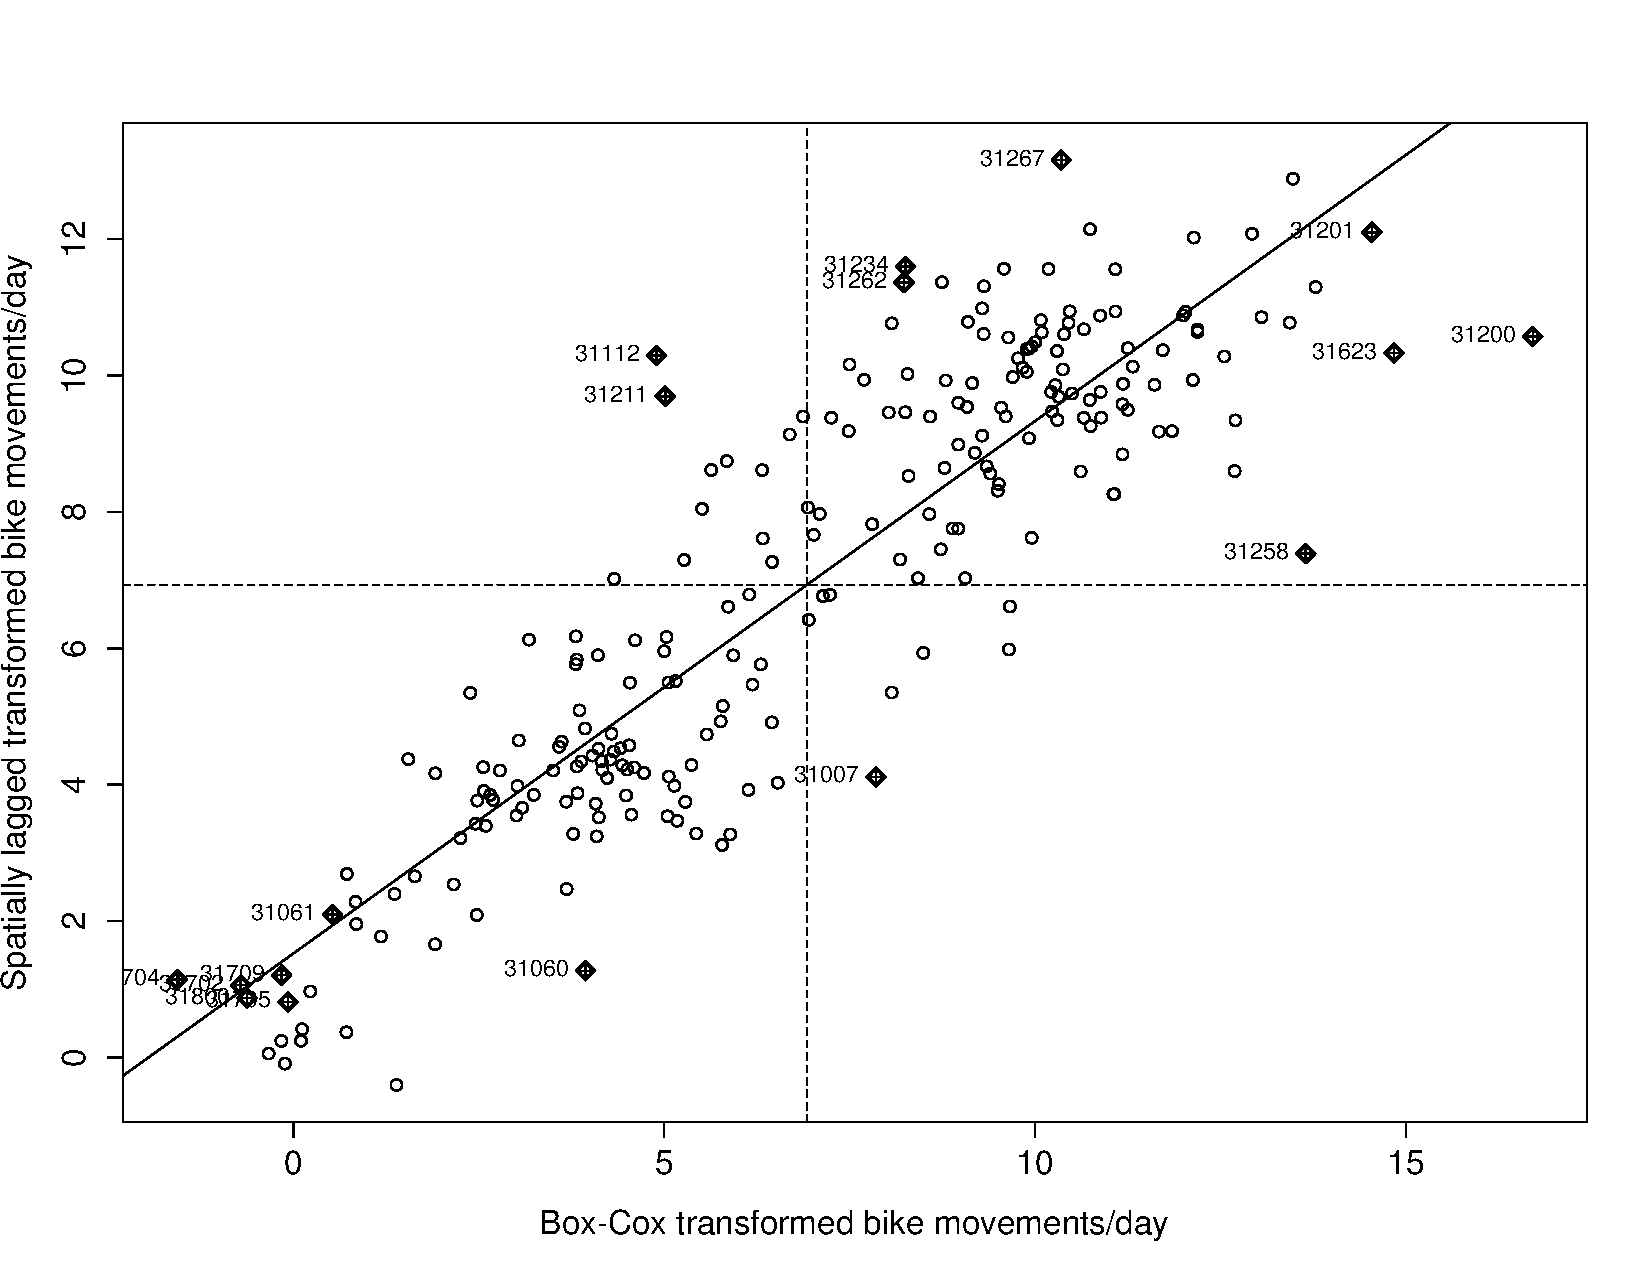
\includegraphics[width=\textwidth]{moran_plot.pdf}
  \caption{\label{fig:moran} Moran plot of station popularity.}
\end{figure}

% Could we test for spatial distribution of Moran outliers?


\subsection{Discussion}

There is significant positive spatial autocorrelation in the
popularities of bikeshare stations. This makes sense intuitively, in
terms of both first- and second-order effects. On the first-order
side, areas with many attractions are likely to have more bike
movements at all stations in the area. On the second-order side, each
trip requires two stations within biking distance of each other; more
stations closer together means more options for trips. One could also
hypothesize an inhibition effect at very fine scales in some
situations: if there are two stations very near each other, but one is
preferable, it may inhibit use of the other one. For example, there
are two stations near the San Francisco train station in the Bay Area
Bikeshare system. One is directly in front of the station, and one is
across the street. It is likely that the one across the street is less
popular because people prefer to use the one in front of the station
when bikes or docks are available. This project did not attempt to
differentiate between first- and second-order effects.

In general, the locations of the influential points are not
surprising. For example, station 31258, one of the stations that is
much more popular than those around it, is located at the Lincoln
Memorial, a popular destination for tourists. It is also a neighbor to
the not-particularly-popular station 31211, despite being separated
from it by freeways; this artificially pulls down the local average and
makes station 31258 more influential. This is a downside of using pure
Euclidean planar geometry to define the neighbor matrix. Station 31211
is itself another good example; it is much less popular than its
neighbors. Some of this is due to the aforementioned connection with
the station at the Lincoln Memorial. This station is also located at
the Kennedy Center, a performing-arts center which is on the Potomac
and separated from much of Washington by Interstate 66. It is not
particularly accessible by bicycle; this is likely the reason it is
not particularly popular. Finally, the aforementioned inhibition
effect of stations very close to each other may be occurring near
DuPont Circle. Station 31200 is located directly on DuPont Circle,
while station 31234 is located about a block away and around a
corner. People, especially tourists, traveling to DuPont Circle likely
ride to the more obvious station; this may inhibit use of the less
obvious station.

\begin{figure}[t]
  \includegraphics[width=\textwidth]{popularities.pdf}
  \caption{\label{fig:map} Map of station popularities and Moran
    influential points.}
\end{figure}

\section{General Discussion and Further Research}

This project found that both time and space exert significant effects
on bikeshare use. The distributions of trips between stations differ
significantly at different times of day. There also tends to be
spatial autocorrelation; popular stations tend to be near each other.

One interesting topic for further research would be to look further
into the origin-destination matrices at different times of day. One
could attempt to determine the direction of movement of the bikes at
different times of day, and the determinants of the movement (for
instance, are people from Metro stations to downtown areas to downtown
areas in the morning due to the commute?). This research would be useful
in that it could inform rebalancing. One team has developed
statistical models for predicting bikeshare station use, but their
approach does not model the flow of bikes between stations because
they did not have full trip data available in Chicago
\autocite{Dempsey2013}. Using origin-destination matrices would be an
alternate way to model bikeshare use.

Another avenue for further research would be to theorize what drives
station popularity. It seems likely that the accessibility of the
station is a driver. For instance, stations more accessible to jobs,
housing or transit stops are likely to be more popular. Additionally,
stations more accessible to other stations may be more popular; the
more stations one can reach by bike from a given location, the more
options one has for potential trips. This could be investigated using
a regression with station popularity as the dependent vuariable and the
various forms of accessibility as independent variables. If the model
proved to be transferable, it would be valuable to planners
implementing new bikeshare systems.

The bikeshare trip data provides a wealth of information for
analysis. Very rarely do researchers have access to complete
origin-destination matrices for a particular mode. This research
confirms the value of geography in explaining the use of this new
transportation tool. Further research could do more with this data,
creating predictive tools to assist bikeshare system operators and
planners.

\clearpage\newpage
\printbibliography

\vspace{25em}

\emph{Copyright © 2013 Matthew Wigginton Conway. CC BY-NC 3.0.}

\newpage
\newgeometry{hmargin=0.5in,vmargin=1in}
\fancyhfoffset[E,O]{0pt}
\appendix
\section{Source Code Listings}

This appendix contains source code listings for the code used in this
project. Data management and retrieval code is primarily Python,
whereas analysis code is written in R. All of the code used in this
project is licensed under the Apache License, is also available at
\url{http://www.github.com/mattwigway/bikeshare-analysis}.

\subsection{Data Management}

Scripts in this section are used to retrieve data from Capital
Bikeshare and process it into a format suitable for analysis.

\subsubsection{fetchData.sh}
\label{fetchData.sh}

This shell script simply calls the other scripts to retrieve and
process the data.

\lstinputlisting[language=sh]{../datamgmt/fetchData.sh}

\subsubsection{csvMerge.py}
\label{csvMerge.py}

This script merges all of the quarterly CSV files into one large CSV
file, merging columns that are the same but have different names in
data files from different time periods.

\lstinputlisting[language=Python]{../datamgmt/csvMerge.py}

\subsubsection{expandFileWithXY.py}
\label{expandFileWithXY.py}

Station locations are not included in the trip history feed, only
their names and numbers. This script takes a trip history file and
adds spatial coordinates of the stations, based on the locations of
stations in the CaBi XML API. It also projects the location to UTM so that
Euclidean geometry can be used in calculations.

\lstinputlisting[language=Python]{../datamgmt/expandFileWithXY.py}

\subsection{Effects of Time on Bikeshare Use}

This section contains scripts used to evaluate the effects of time on
bikeshare use.

\subsubsection{periods.R}
\label{periods.R}

This code simply defines how the time periods are coded. They are
stored as single numbers in the file to reduce the file size.

\lstinputlisting{../analysis/periods.R}

\subsubsection{load\_data.R}
\label{load_data.R}

This code loads and filter the trip data from CaBi, dropping trips
over 20 km or 24 hours.

\lstinputlisting{../analysis/load_data.R}

\subsubsection{labeling.R}
\label{labeling.R}

This code takes the Capital Bikeshare trip data, cleaned by the above
scripts, and labels it based on trip start time period.

\lstinputlisting{../analysis/labeling.R}

\subsubsection{relabel.R}
\label{relabel.R}

This script calculates test statistics for the observed distribution
of trips then randomizes the distribution of trips to time periods,
conducting a Monte Carlo simulation to determine the p-value of the
observed trip distribution.

\lstinputlisting{../analysis/relabel.R}

\subsection{Effects of Space on Bikeshare Use}
\subsubsection{morans\_i.R}
\label{morans_i.R}

This script was used to calculate Moran's $I$ to calculate how
spatially autocorrelated the popularity of bikeshare stations is.

\lstinputlisting{../analysis/morans_i.R}

\subsubsection{ui.R}
\label{ui.R}

This script is the UI for the Shiny application used to evaluate the
link threshold distance (see figure \ref{fig:shiny}).

\lstinputlisting{../analysis/cull_links_shiny/ui.R}

\subsubsection{server.R}
\label{server.R}

This is the server component of the Shiny application used to evaluate
the link threshold distance.

\lstinputlisting{../analysis/cull_links_shiny/server.R}

\end{document}
